\documentclass{article}
\usepackage[T1]{fontenc}
\usepackage{lmodern}
\usepackage{graphicx}
\usepackage{amsmath,amssymb}
\usepackage[a4paper,margin=2cm]{geometry}
\usepackage[absolute,overlay]{textpos}
\setlength{\TPHorizModule}{1mm}
\setlength{\TPVertModule}{1mm}
\usepackage[indonesian]{babel}
\usepackage{hyperref}
\setlength{\emergencystretch}{2em}
% unit: Halaman 6

\begin{document}

% === Halaman 6 (llm) ===

\vspace{166.32mm}

\textbf{Tabel} Frekuensi kemunculan (relatif) huruf-huruf dalam teks Bahasa Inggris (sampel mencapai 300.000 karakter di dalam sejumlah novel dan suratkabar)

% deskripsi: Tabel distribusi frekuensi relatif huruf-huruf alfabet Inggris.
% bbox normalisasi: [0.0300, 0.3000, 0.5300, 0.8600]
\begin{textblock*}{105.00mm}(6.30mm,89.10mm)
\noindent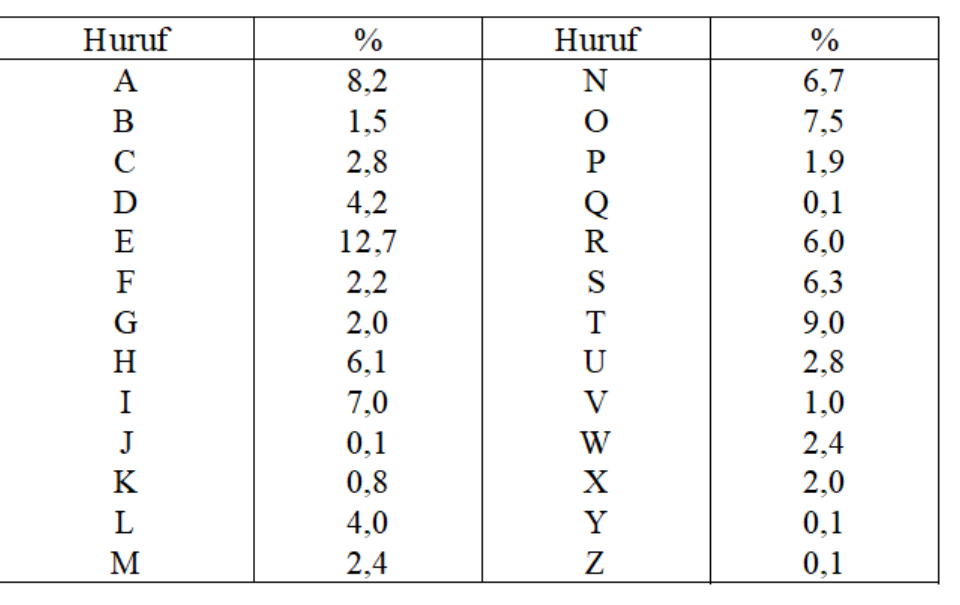
\includegraphics[width=105.00mm,height=166.32mm]{../../images/llm/page_006_img_01.png}%
\end{textblock*}

% deskripsi: Grafik batang yang menunjukkan frekuensi relatif kemunculan setiap huruf alfabet Inggris.
% bbox normalisasi: [0.5600, 0.2100, 0.9600, 0.9100]
\begin{textblock*}{84.00mm}(117.60mm,62.37mm)
\noindent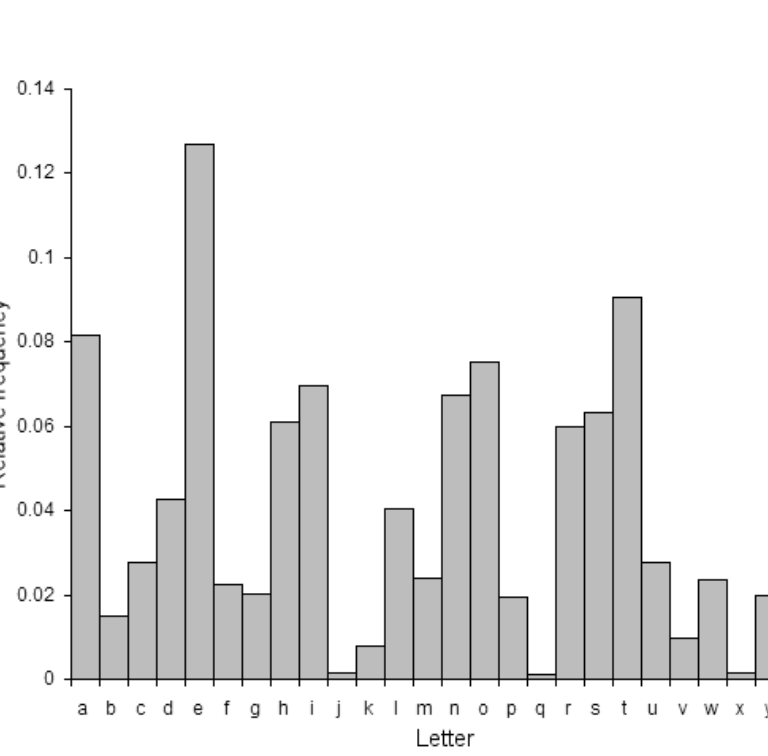
\includegraphics[width=84.00mm,height=207.90mm]{../../images/llm/page_006_img_02.png}%
\end{textblock*}

\end{document}
